\documentclass[compress,noflama,nosectionpages]{beamer}
%--------------------------------------------------------------------------
% Common packages
%--------------------------------------------------------------------------

%\usepackage[inline]{enumitem}%jsta added
\usepackage[normalem]{ulem}%jsta added
\usepackage{hyphenat}%jsta added
\usepackage{rotating}%jsta added
\usepackage{graphicx}
\usepackage{multicol}
\usepackage{tabularx,ragged2e}
\usepackage{booktabs}
\usepackage{listings}
\lstset{ %
language=[LaTeX]TeX,
basicstyle=\normalsize\ttfamily,
keywordstyle=,
numbers=left,
numberstyle=\tiny\ttfamily,
stepnumber=1,
showspaces=false,
showstringspaces=false,
showtabs=false,
breaklines=true,
frame=tb,
framerule=0.5pt,
tabsize=4,
framexleftmargin=0.5em,
framexrightmargin=0.5em,
xleftmargin=0.5em,
xrightmargin=0.5em
}

%--------------------------------------------------------------------------
% Load theme
%--------------------------------------------------------------------------
\usetheme{hsrm}


%------jsta test
% \setbeamertemplate{navigation symbols}{}
%  \makeatletter\
% \setbeamertemplate{footline}
% {
%  \pgfuseshading{beamer@barshade}
%  \ifbeamer@sb@subsection
%  \vskip-9.75ex
%  \else
%  \vskip-7ex
%  \fi
%  \begin{beamercolorbox}[ignorebg,ht=2.25ex,dp=3.75ex]{section in head/foot}
%  \insertnavigation{\paperwidth}
%  \end{beamercolorbox}
%  \ifbeamer@sb@subsection
%  \begin{beamercolorbox}[ignorebg,ht=2.125ex,dp=1.125ex,leftskip=.3cm,rightskip=.3cm plus1fil]{subsection in head/foot}
%  \usebeamerfont{subsection in head/foot}\inserctsubsectionhead
%  \end{beambercolorbox}
%  \fi
%  }
%  \setbeamertemplate{headline}{
%  \hskip1em\usebeamercolor[fg]{navigation symbols dimmed}
%  \insertslidenavigationsymbol
%  \insertframenavigationsymbol
%  \insertsectionnavigationsymbol
%  \insertsubsectionnavigationsymbol
%  \insertdocnavigationsymbol
%  \insertbackfindforwardnavigationsymbol
%  }
% \makeatother


%------

%jsta commented out%\usepackage{dtklogos} % must be loaded after theme
\usepackage{tikz}
\usetikzlibrary{mindmap,backgrounds}

%--------------------------------------------------------------------------
% General presentation settings
%--------------------------------------------------------------------------
\title{\nohyphens{Fine-scale spatial patterning \protect\\ of phytoplankton abundance \protect\\ in a coastal estuary}}
\subtitle{\nohyphens{ }}
\date{August 2016}
\author{{\Medium Joseph Stachelek}, Christopher Madden, Stephen P. Kelly, Michelle Blaha}
\institute{{\Medium Michigan State University} South Florida Water Management District}

%--------------------------------------------------------------------------
% Notes settings
%--------------------------------------------------------------------------
\setbeameroption{show notes}

\begin{document}
%--------------------------------------------------------------------------
% Titlepage
%--------------------------------------------------------------------------

\maketitle

%\begin{frame}[plain]
%  \titlepage
%\end{frame}


%--------------------------------------------------------------------------
% Content
%--------------------------------------------------------------------------
\section{Introduction}
\subsection{Introduction}

% \begin{frame}{Why describe phytoplankton distributions?}
% 	Eutrophication \\
% 	Water Management \\
% \end{frame}

\begin{frame}{How can we describe phytoplankton distributions?}

	\begin{centering}
		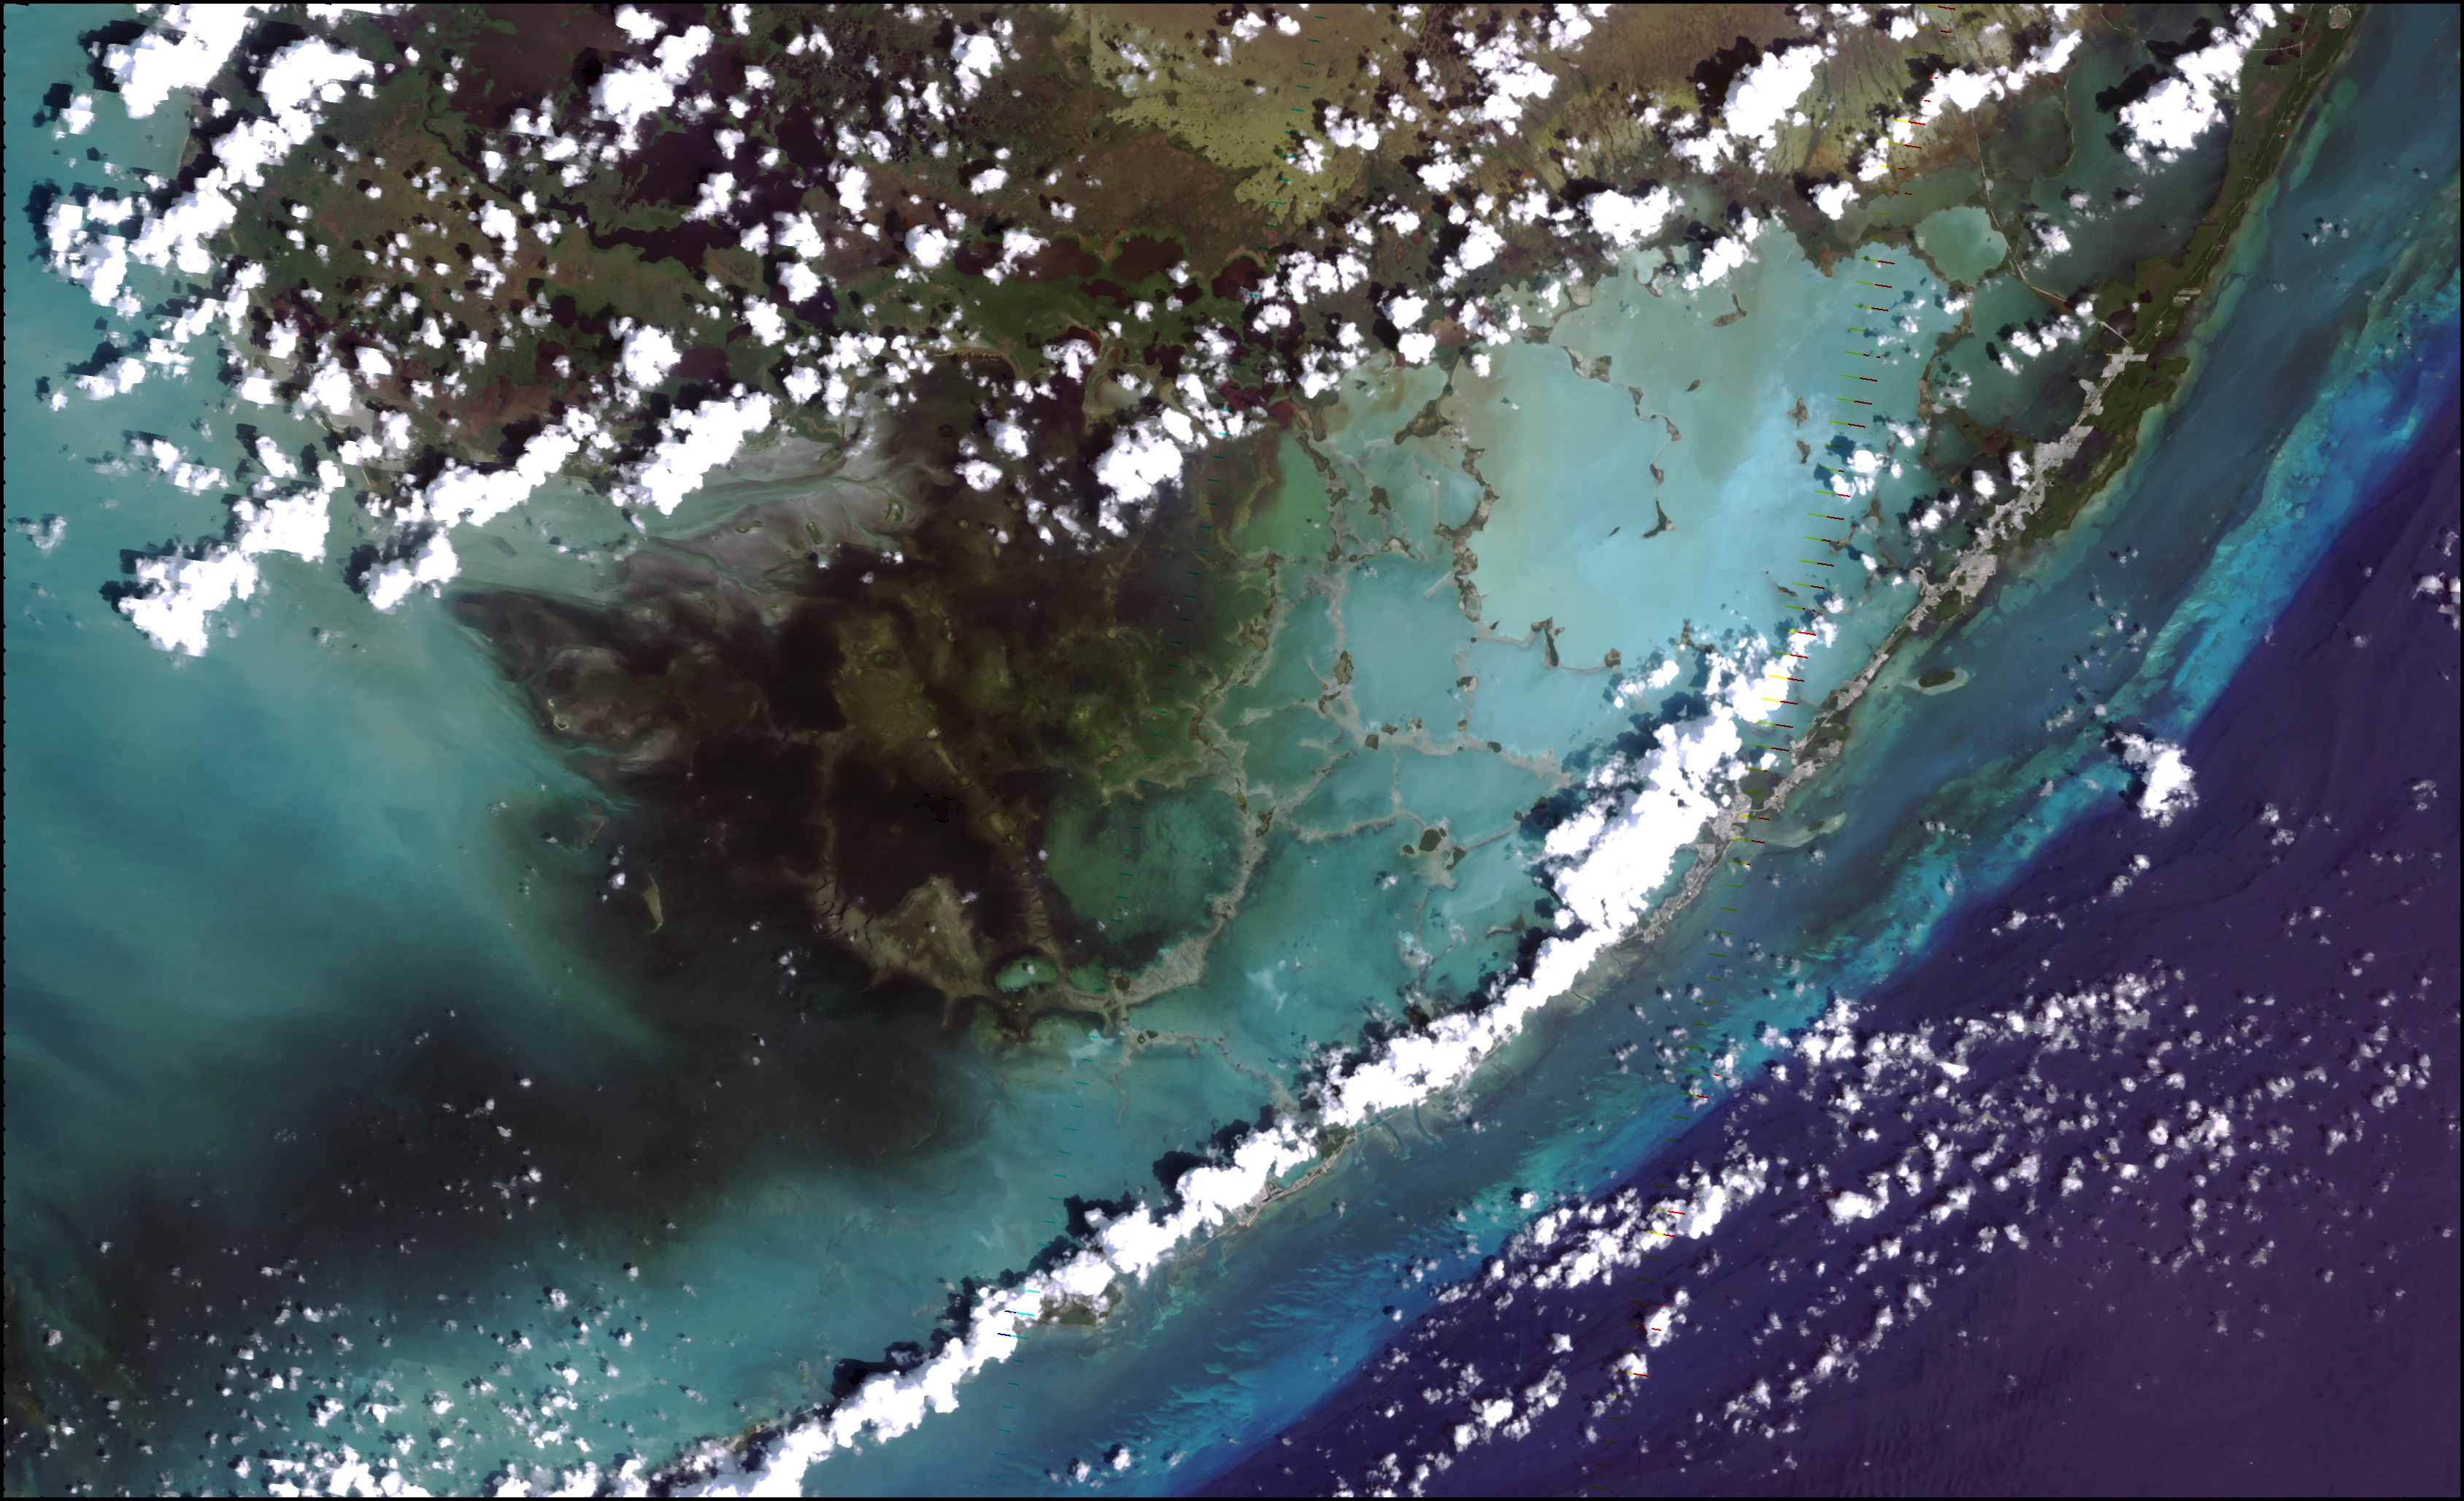
\includegraphics[height=6cm,keepaspectratio=true]{images/landsat_border.jpg}\\
	\end{centering}

\end{frame}

\begin{frame}{The Discrete Approach}
	\begin{columns}
		\begin{column}[c]{5.5cm}
			\begin{center}
			Bay-Wide Network\\ (Monthly, 1993 - 2015)
			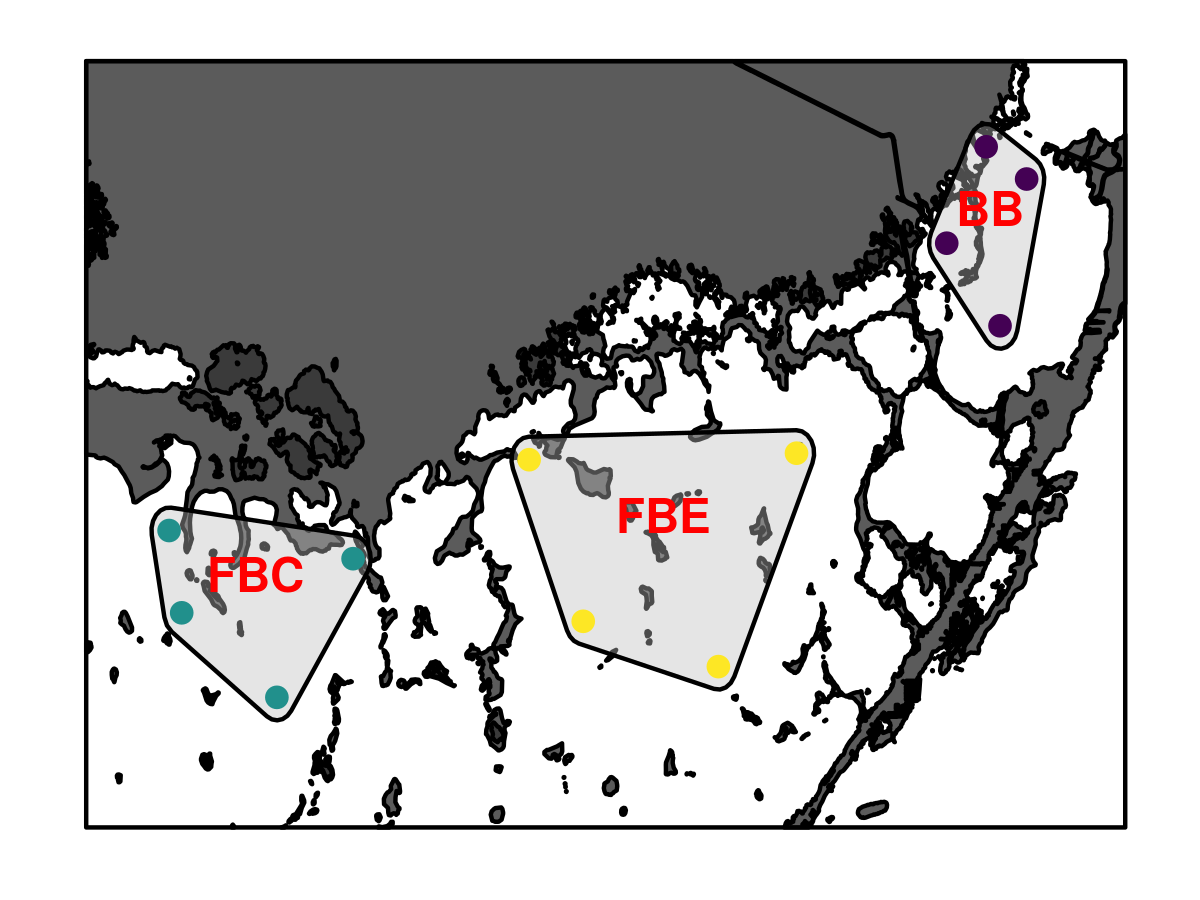
\includegraphics[height=4.7cm,clip=true,trim = 0mm 0mm 0mm 0mm,keepaspectratio=true]{figures/fbmap_wqmn.png}%
			\end{center}
		\end{column}
	
		\begin{column}[c]{6cm}
			\begin{center}
			Coastal Network\\ (Quarterly, 2008 - 2015)
			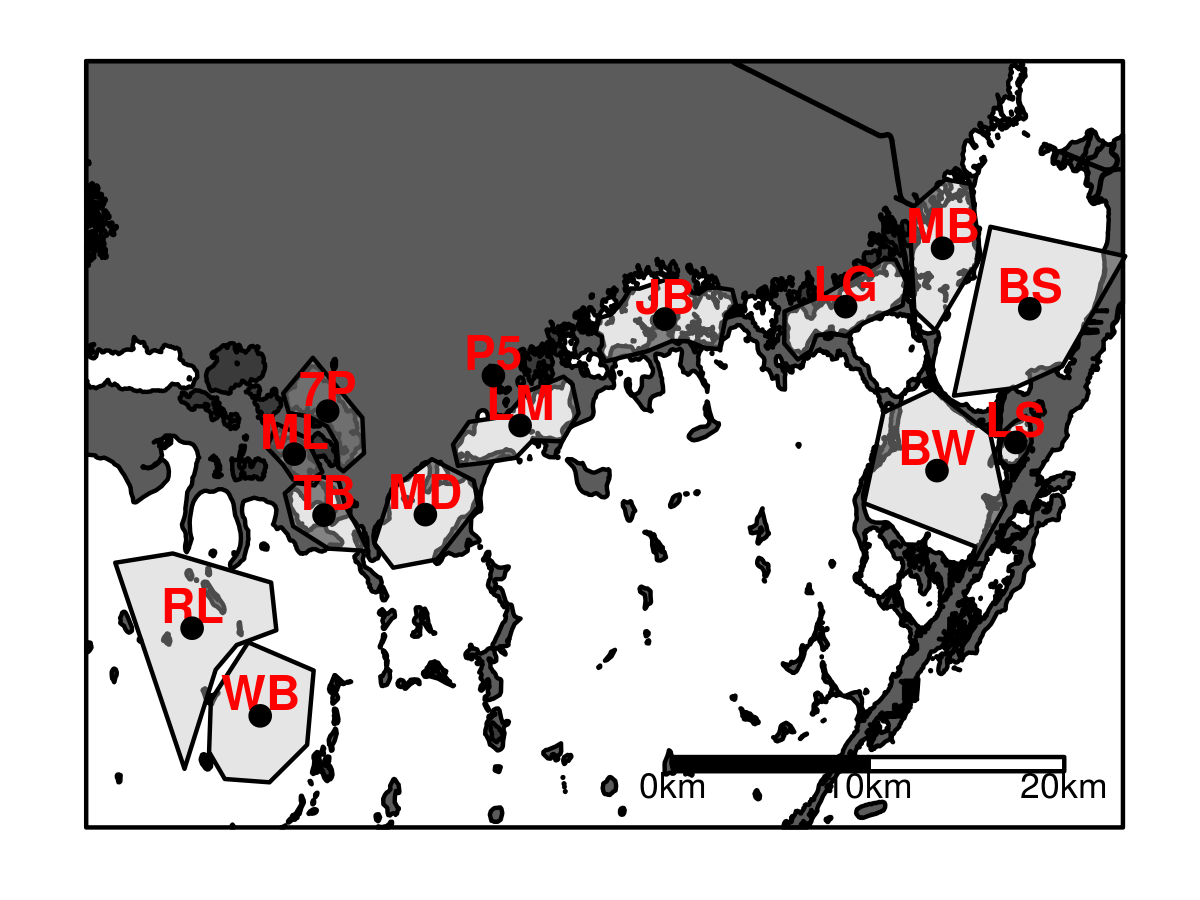
\includegraphics[height=4.7cm,clip=true,trim = 0mm 0mm 0mm 0mm,keepaspectratio=true]{figures/fbmap_dflow.png}%
			\end{center}
		\end{column}
	\end{columns}
\end{frame}

\begin{frame}{Bay-Wide Network}
			\begin{columns}
				\begin{column}[c]{6cm}
					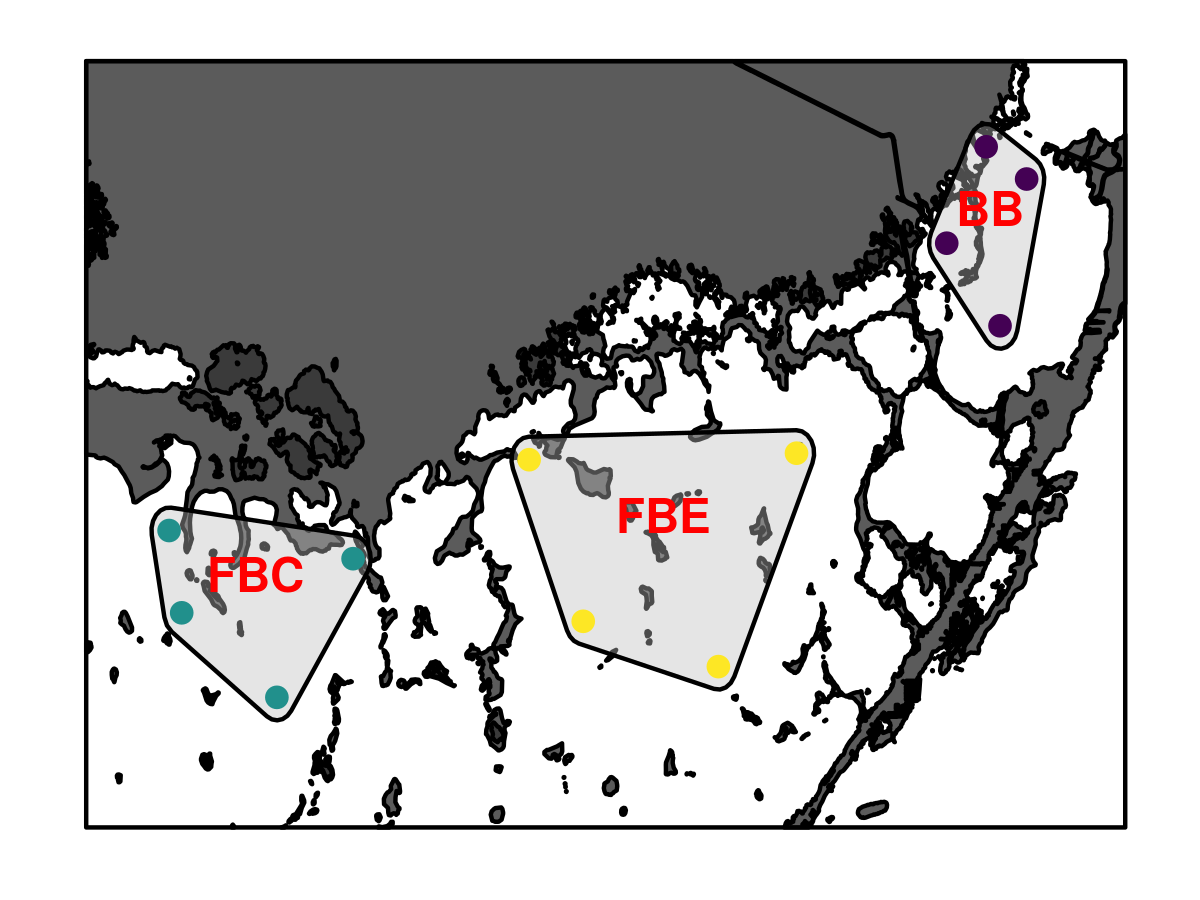
\includegraphics[height=4.5cm,clip=true,trim = 0mm 0mm 0mm 0mm,keepaspectratio=true]{figures/fbmap_wqmn.png}%
				\end{column}
				
				\begin{column}[c]{6.0cm}
				\begin{centering}
					\begin{tikzpicture}
						\node[anchor=south west,inner sep=0] at (0,0) {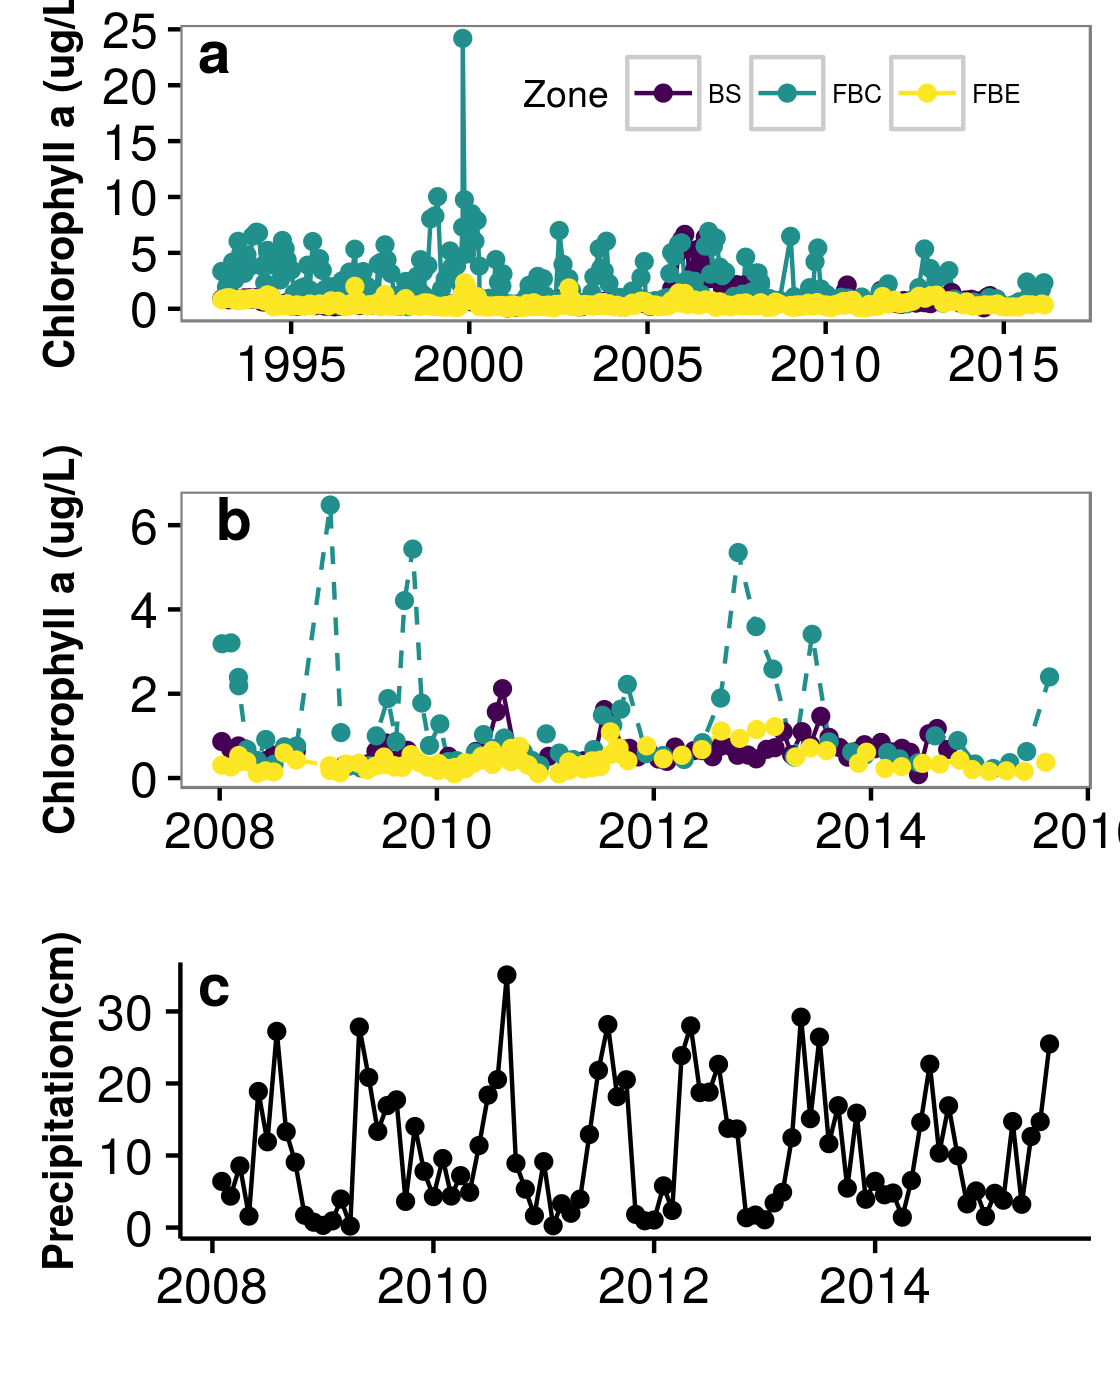
\includegraphics[width=5.9cm]{figures/chltimeseries.png}};
						% \draw[help lines,xstep=1,ystep=1](0,0) grid (5.9,7.4);
						% \foreach \x in {0,1,...,6}{ \node [anchor=north] at (\x,0) {\x};}
						% \foreach \y in {0,1,...,7}{ \node [anchor=east] at (0,\y) {\y};}
					 	% \draw[red,thick, rounded corners](3.3,5.8) rectangle (4.1,6.3);
					 	\draw[red,thick, rounded corners](1.9,3.2) rectangle (2.4,4.8);
					 	\draw[red,thick, rounded corners](3.6,3.2) rectangle (4.6,4.8);
					\end{tikzpicture}
					\end{centering}
				\end{column}
			\end{columns}
			\vspace{-3em}
		\end{frame}

\begin{frame}{Coastal Network}
			\begin{columns}
				\begin{column}[c]{5.3cm}
					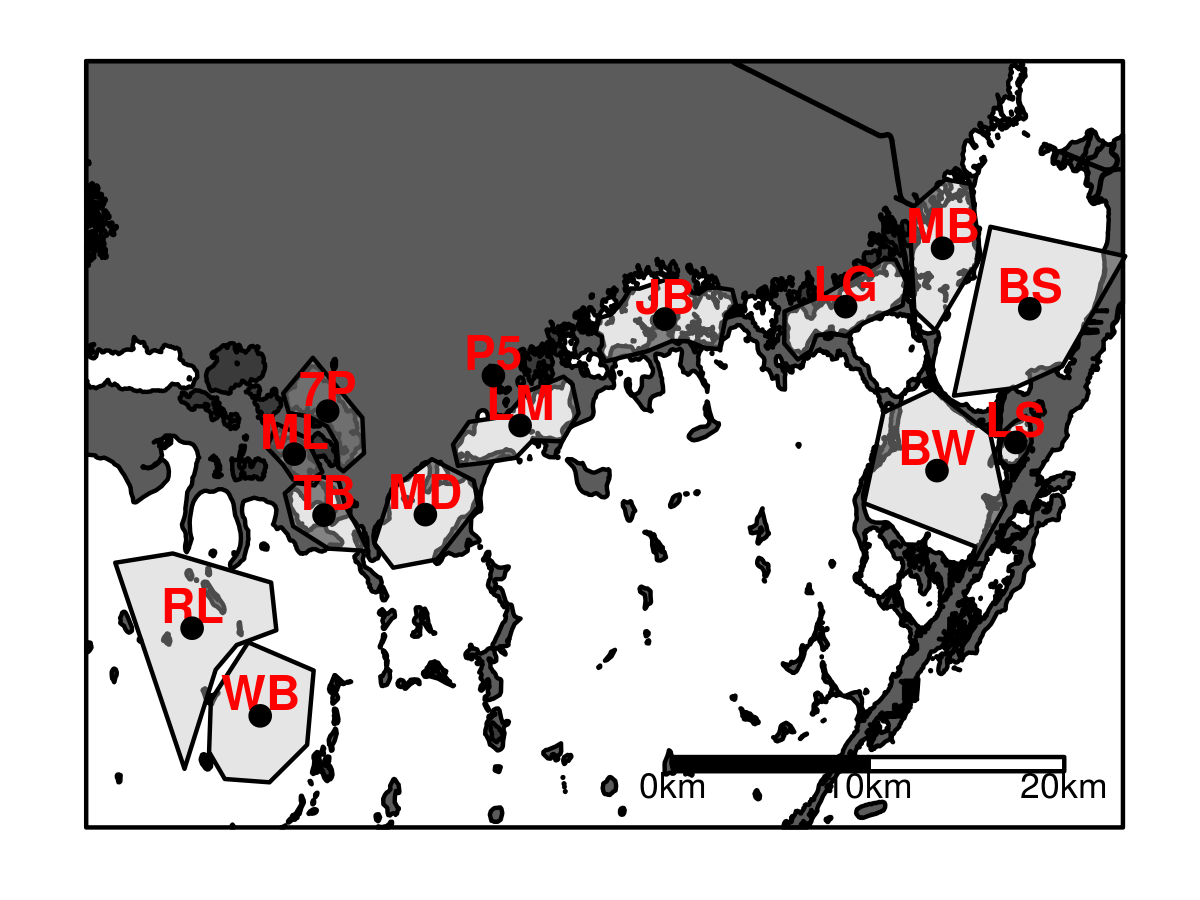
\includegraphics[height=4.5cm,clip=true,trim = 0mm 0mm 0mm 0mm,keepaspectratio=true]{figures/fbmap_dflow.png}%
				\end{column}
				
				\begin{column}{7.0cm}
					\vspace{1em}
					\begin{center}
					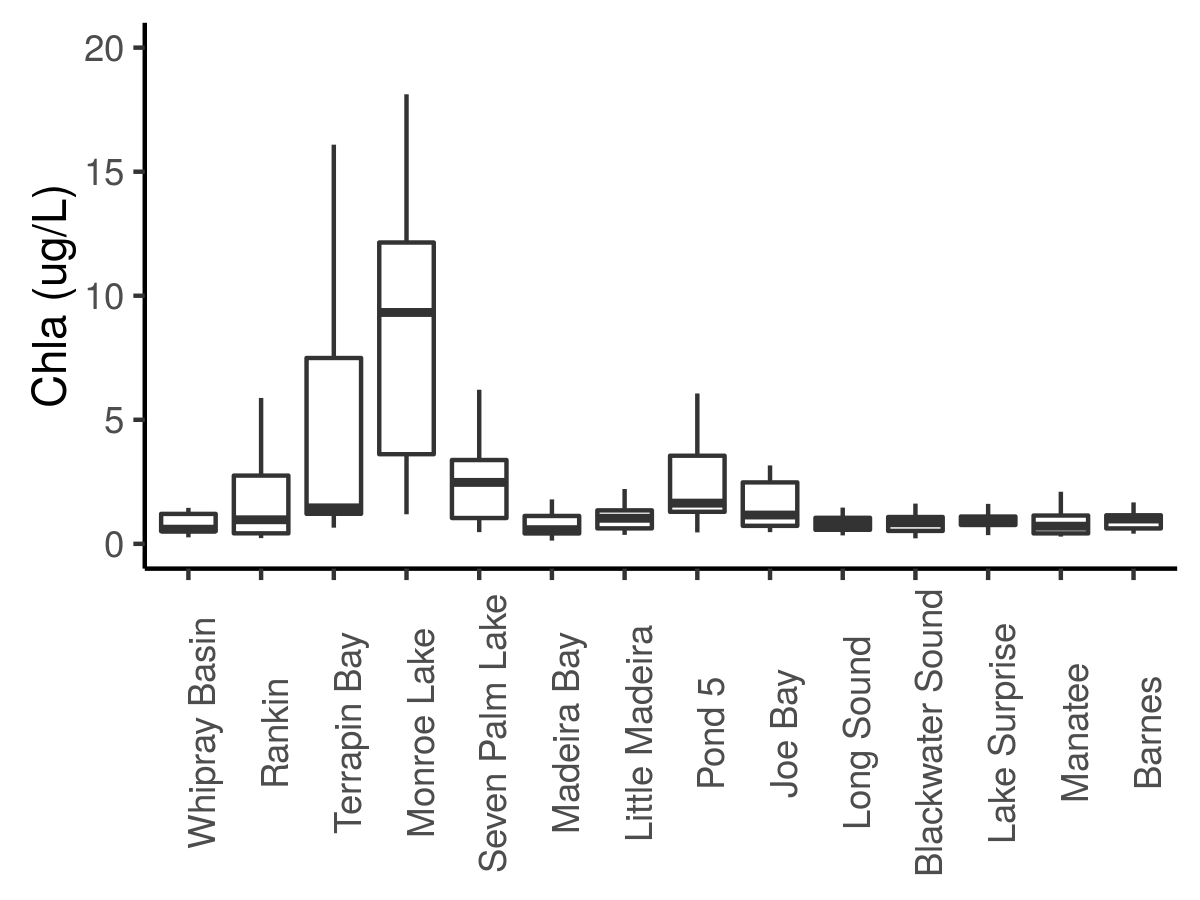
\includegraphics[height=5cm,clip=true,trim = 0mm 0mm 0mm 0mm,keepaspectratio=true]{figures/chlboxplot.png}%
					\end{center}
				\end{column}
			\end{columns}
\end{frame}

\begin{frame}{What do we miss with the Discrete Approach?}
\vspace{8pt}
	\begin{columns}
		\begin{column}[c]{6cm}
	  	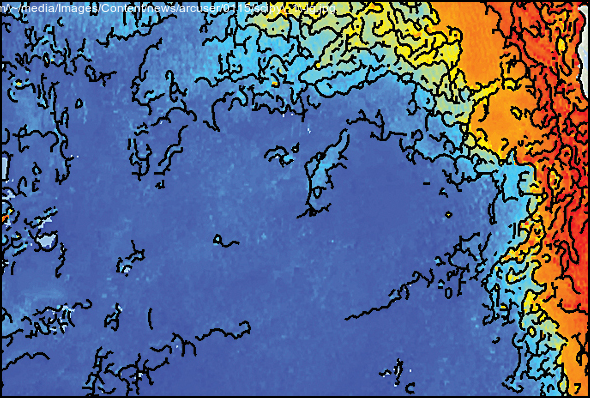
\includegraphics[height=4.1cm,clip=true,trim = 0mm 0mm 0mm 0mm,keepaspectratio=true]{images/scipy_border.png}%
	  	\vspace{3pt}
	  	\begin{itemize}
	  		\item{Spatial Gradients}
	  	\end{itemize}
	  	%\vspace{25pt}
	  	%{\fontsize{3pt}{3pt}\selectfont http\://www.esri.com/\~/media/Images/Content/news/arcuser/0115/scipy\_1\-lg.jpg}\normalsize
		\end{column}
		\begin{column}[c]{6cm}
			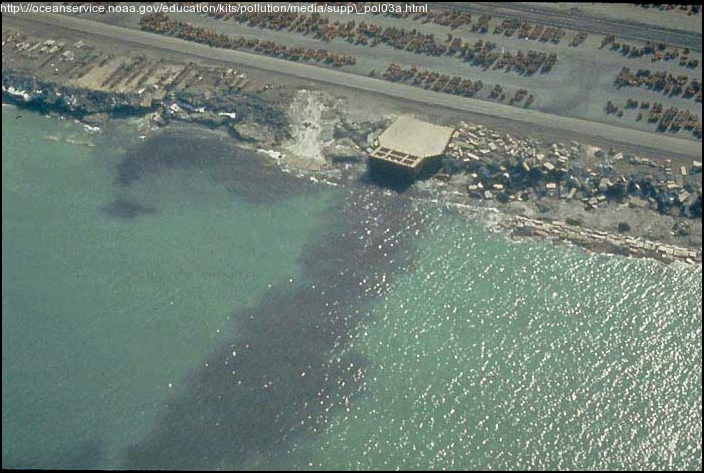
\includegraphics[height=4.1cm,keepaspectratio=true]{images/pointsource_border.png}%
			\vspace{3pt}
			\begin{itemize}
	  		\item{Point Source Extent}
	  	\end{itemize}
	  	%\vspace{25pt}
	  	%{\fontsize{3pt}{3pt}\selectfont http\://oceanservice.noaa.gov/education/kits/pollution/media/supp\_pol03a.html}\normalsize
		\end{column}
	\end{columns}
     
\end{frame}


\begin{frame}[label=data]{An Alternative - The Underway Approach}
  \begin{columns}
    \begin{column}{5.6cm}
      \begin{itemize}
        \item{Quarterly surveys}\vspace{15pt}\\
        \item{Measurements every 50m}\vspace{15pt}\\         \item{Emphasis on freshwater discharge}
      \end{itemize}
    \end{column}
    \begin{column}{6.8cm}
    	\begin{picture}(60,60)(0,-18)
      	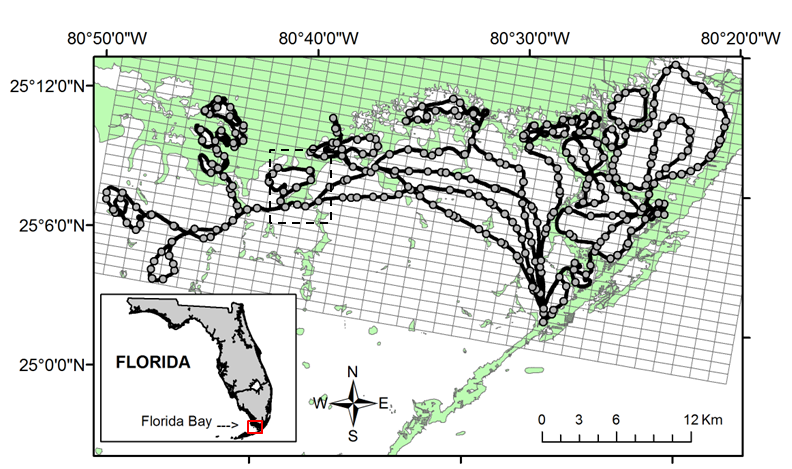
\includegraphics[width=6.5cm,keepaspectratio=true]{figures/sm-figure0.png}
      \end{picture}
      \begin{picture}(80,80)(45,80)
      	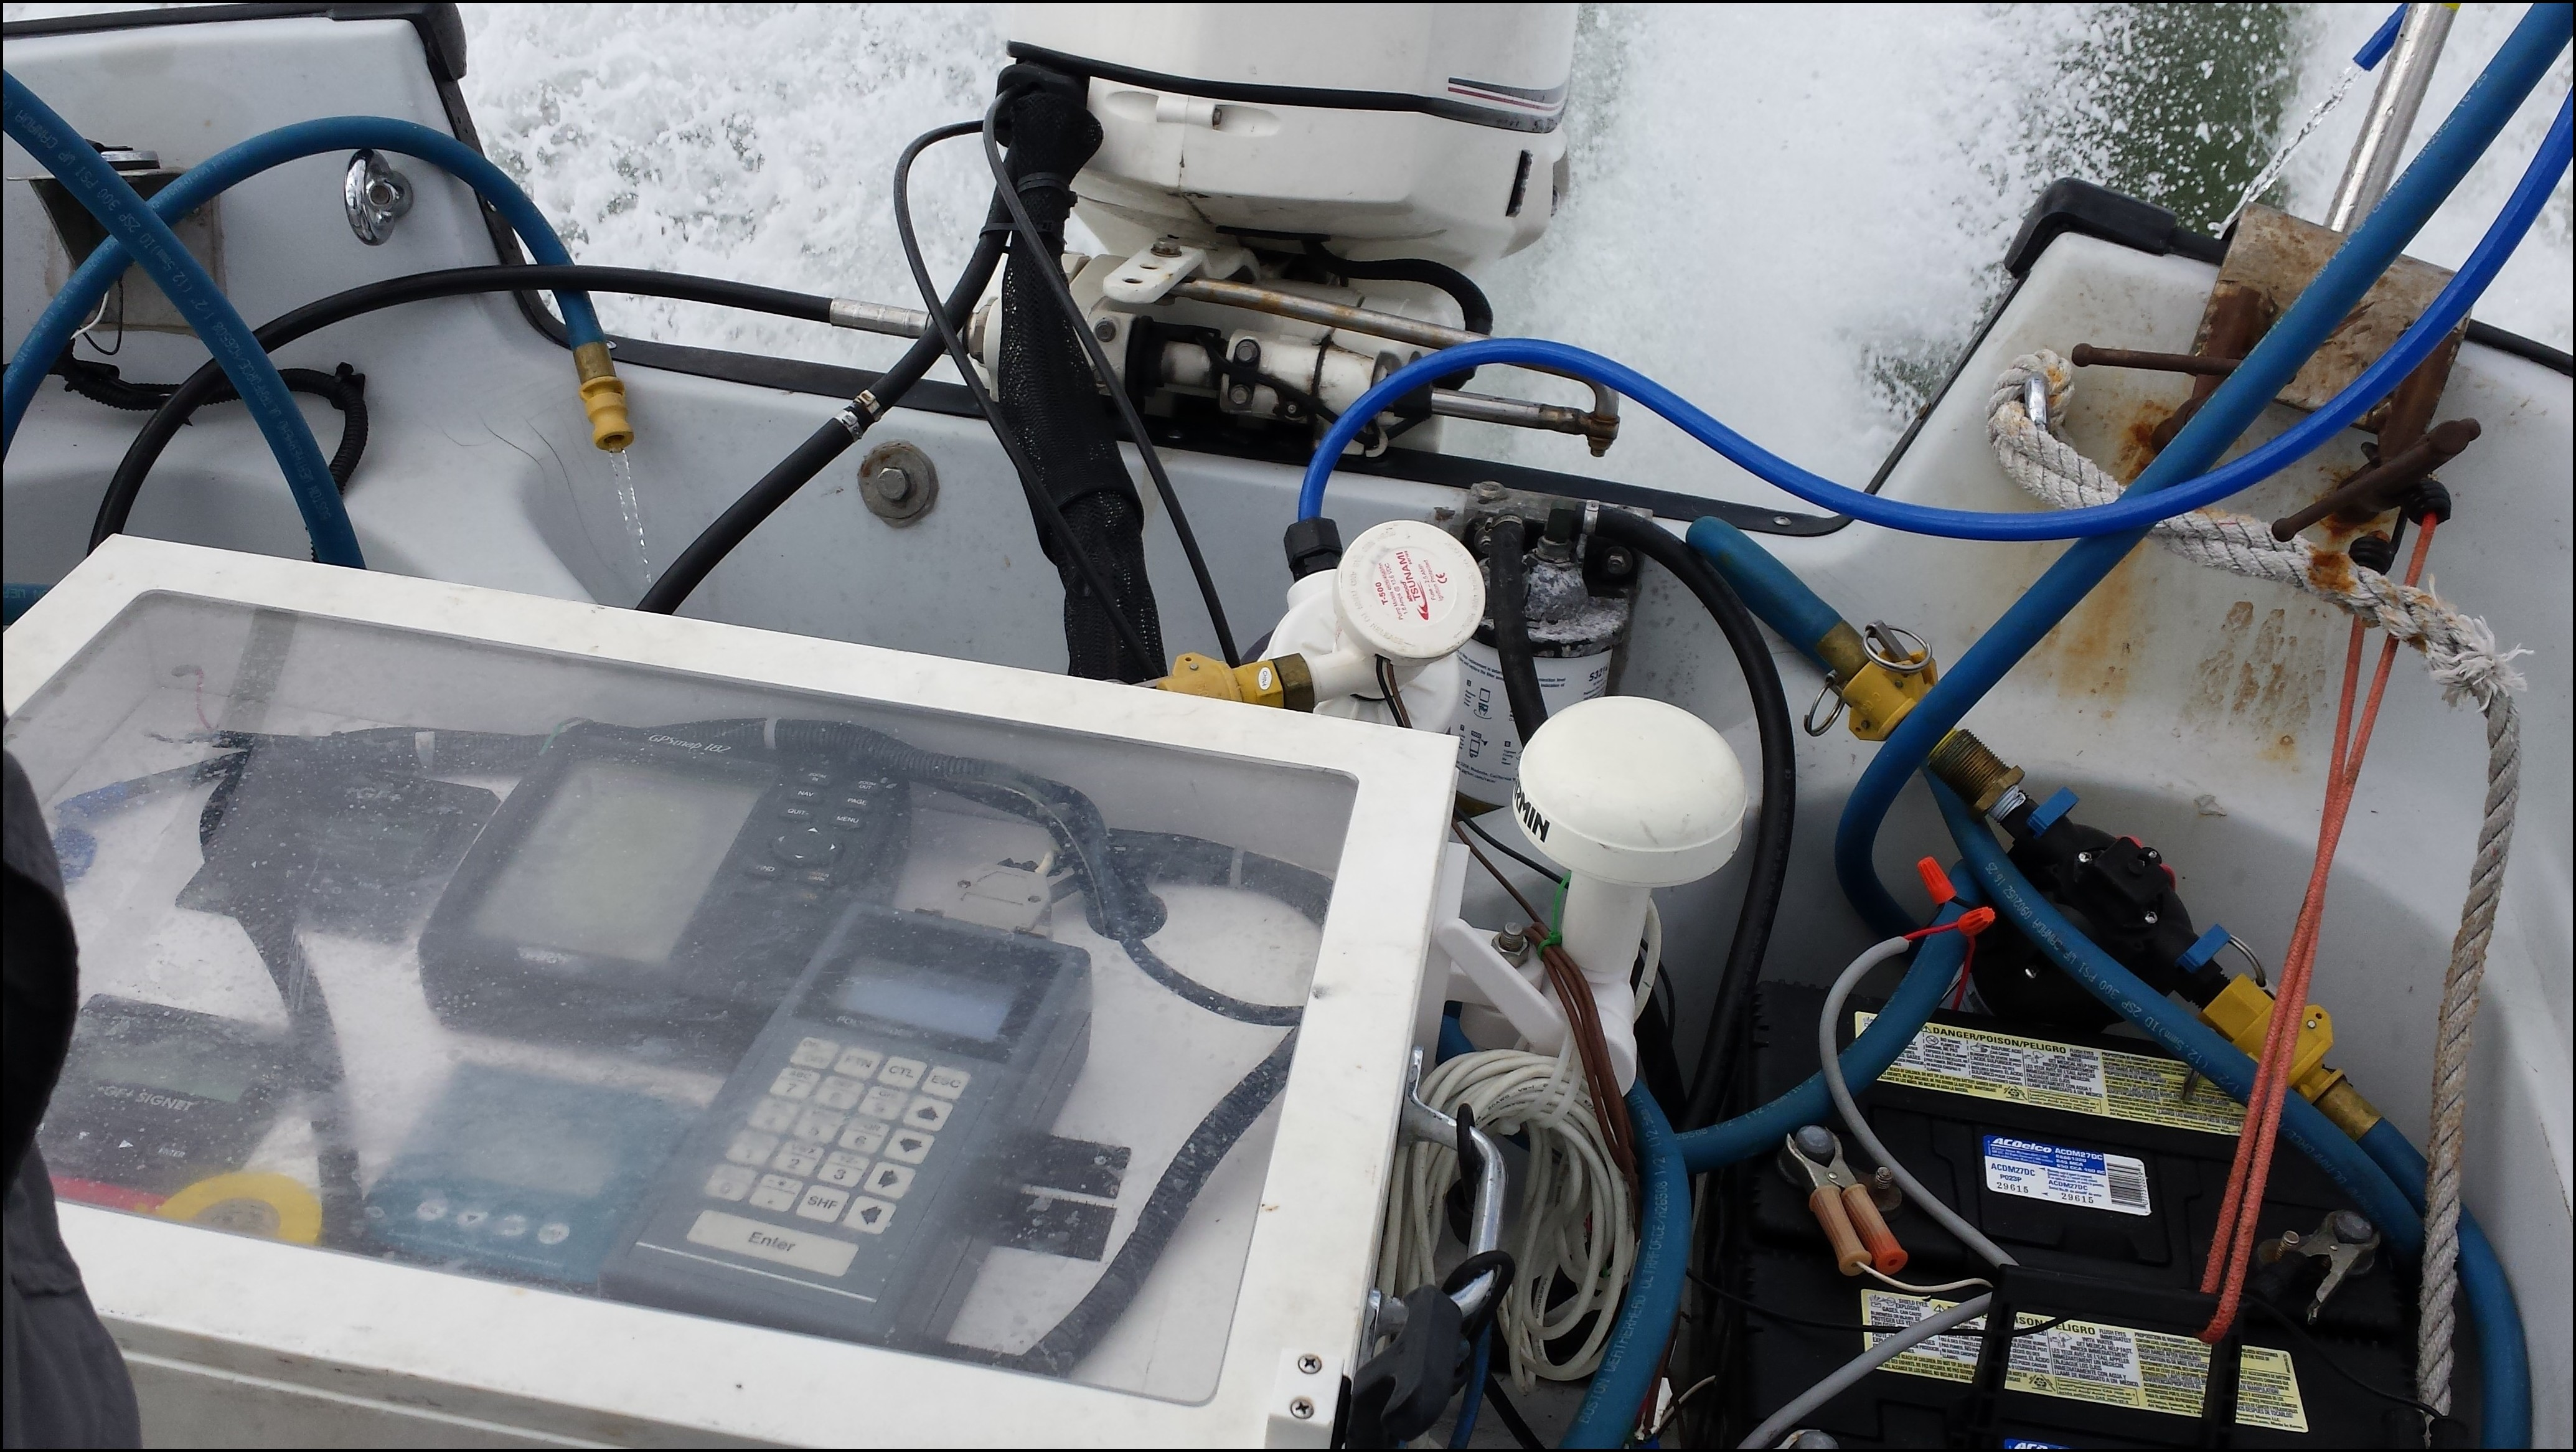
\includegraphics[width=5.5cm,keepaspectratio=true]{images/dflow_border.jpg}
      \end{picture}
    \end{column}
  \end{columns}
\end{frame}

\begin{frame}{Chlorophyll Modelling\textsuperscript{1 2}}
\vspace{2pt}
	\begin{columns}
		\begin{column}{5cm}
			{\footnotesize
			\begin{tabular}{| l | l |}
				\hline
				Instrument Package & Parameter \\ \hline
				Optical 1 & CDOM \\
				... & Chlorophyll \\ \hline
				Optical 2 & CDOM \\
				... & Chlorophyll \\
				... & Phycocyanin \\
				... & Phycoerytherin \\ \hline
			\end{tabular}
			}
			\end{column}
			\begin{column}{4.5cm}
				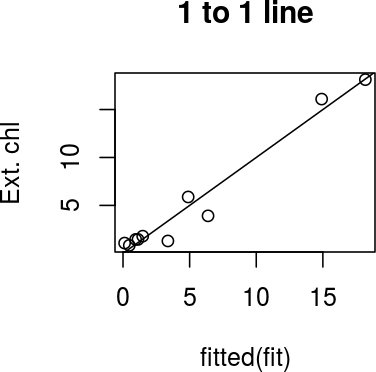
\includegraphics[width=4.2cm,keepaspectratio=true]{figures/chl_onetoone.png}
			\end{column}
	\end{columns}
	\small
	\texttt{DataflowR::chlcoef(201509)}\\
	\texttt{> Initial correlation matrix}\\
	\texttt{> MLR with all variables...}\\
	\texttt{> Checking for redundancy in variable pairs}\\
	\texttt{> Generate AIC for candidate models}\\
	\texttt{> Checking VIF...}

\tiny{\phantom{\footnote{Sepp\"{a}l\"{a} et al. 2007 \textsuperscript{2}Venables and Ripley 2002}}}
\end{frame}

\begin{frame}{What did we learn from chl modelling?}
%\vspace{1em}
	\begin{columns}
		\begin{column}[c]{6cm}
			\vspace{-2em}
			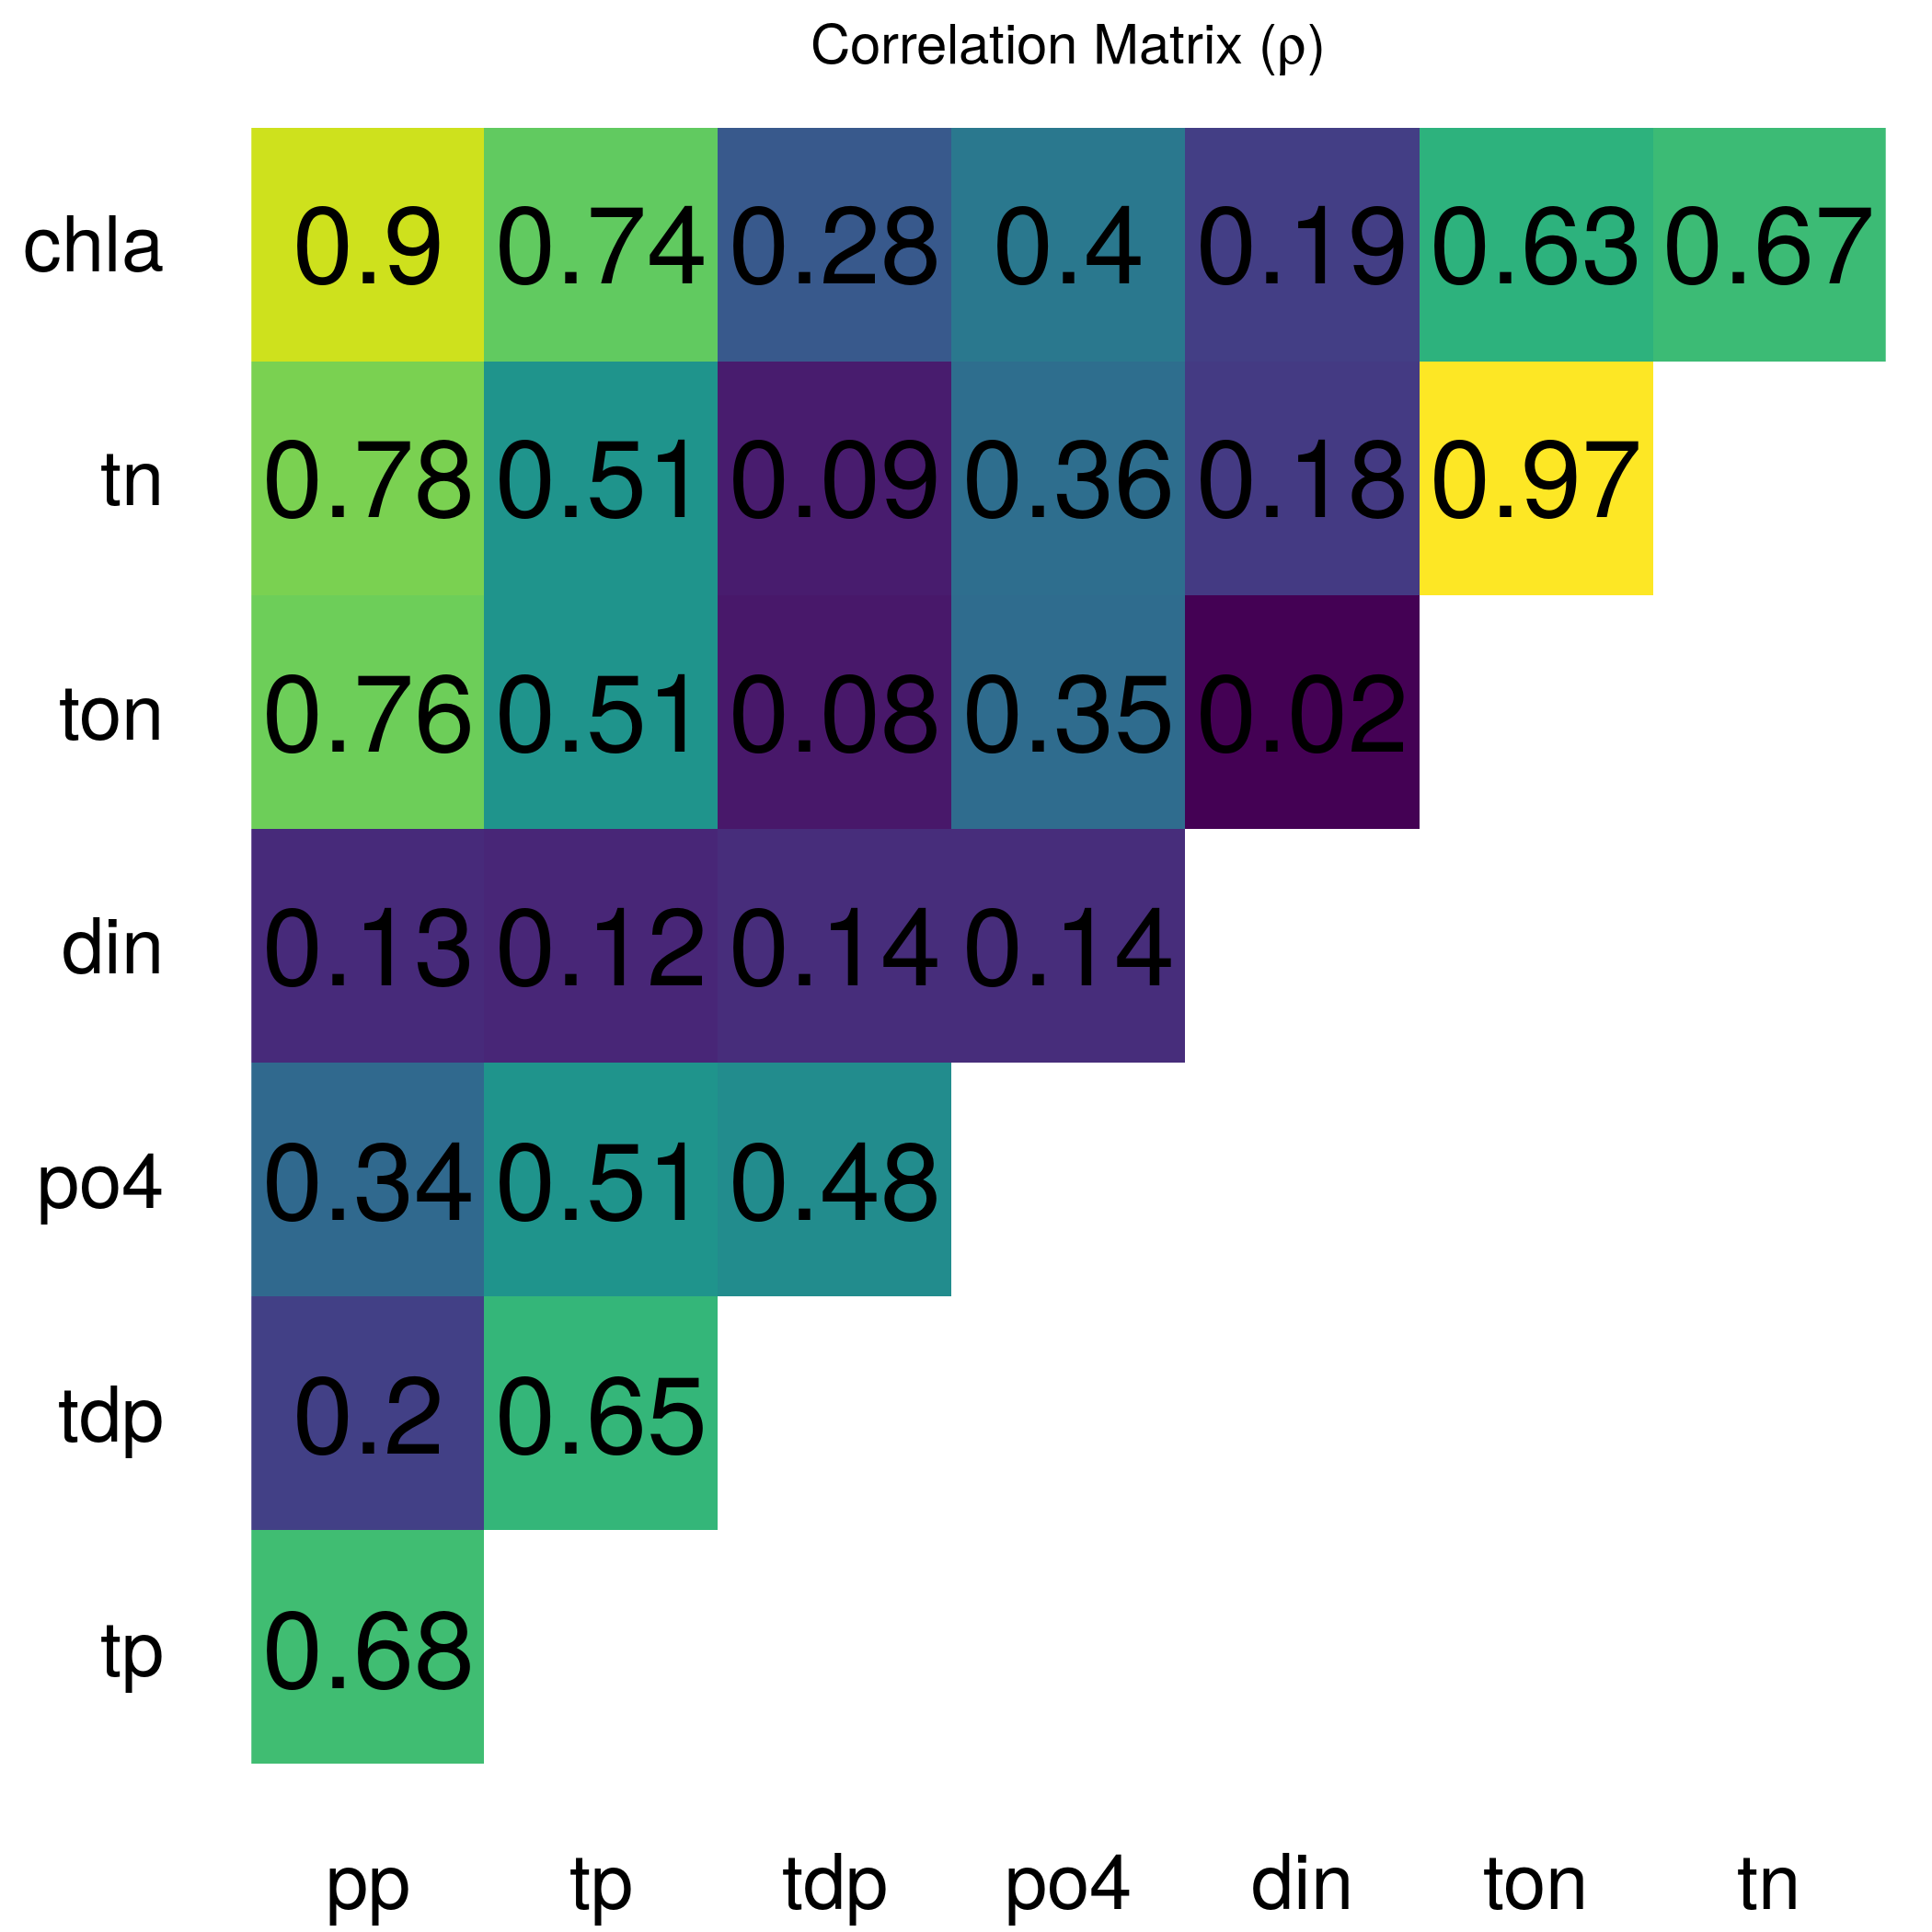
\includegraphics[width=6.2cm,keepaspectratio=true]{figures/chlcor_heatmap.png}
		\end{column}
		\begin{column}[c]{6cm}
			\begin{center}
			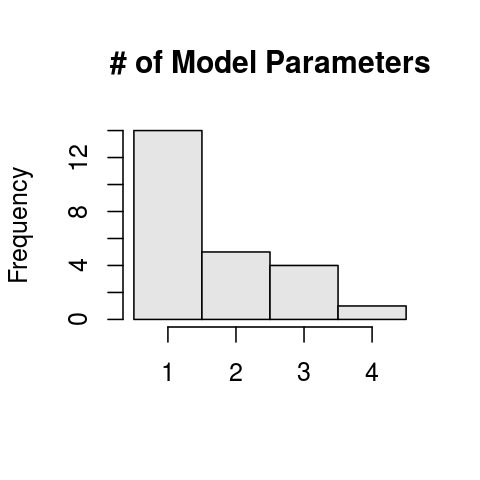
\includegraphics[width=4.2cm,keepaspectratio=true,clip=TRUE,trim= 0mm 5mm 0mm 7mm]{figures/modelparam_counts.png}\\
			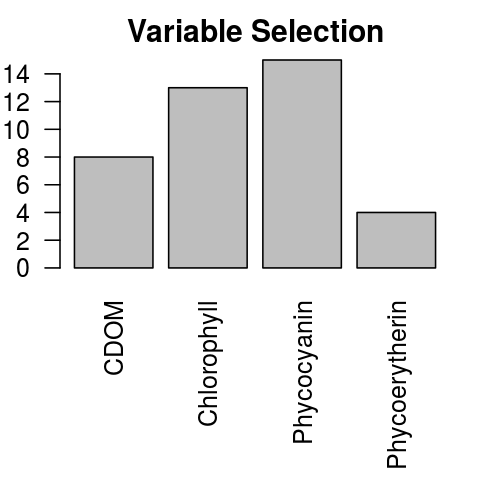
\includegraphics[width=4.2cm,keepaspectratio=true,clip=TRUE,trim= 0mm 0mm 0mm 2mm]{figures/modelparam_hist.png}
			\end{center}
		\end{column}
	\end{columns}
\end{frame}

\begin{frame}{Inverse Path Distance Weighting (IPDW)}
	As the crow flies or as the fish swims?\footnote{Little et al. 1997}\footnote[frame]{Suominen et al. 2010}
	\vspace{6pt}
 	\begin{columns}
   	\begin{column}{6.8cm}
     	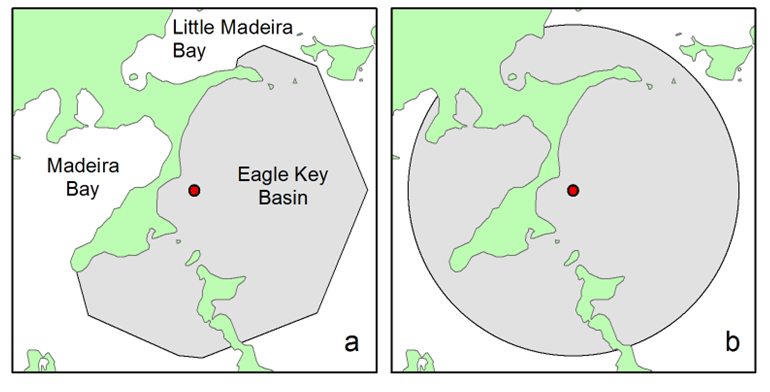
\includegraphics[width=6.8cm,keepaspectratio=true,clip=true,trim= 0mm 0mm 0mm 0mm]{figures/sm-figure1.png}
 		\end{column}

 		\begin{column}{5.4cm}
     	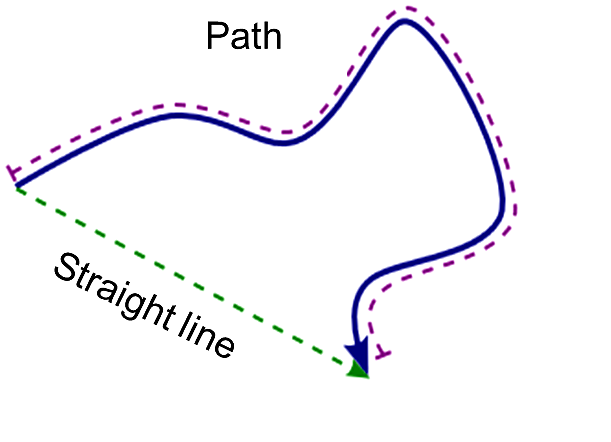
\includegraphics[width=4.8cm,keepaspectratio=true]{images/Picture1.png}
%     	\begin{align*}
%     		V = \frac{\sum\limits_{i=1}^n v_i \frac{1}{d_i^p}}{\sum\limits_{i=1}^n \frac{1}{d_i^p}}
%     	\end{align*}
   	\end{column}
 \end{columns}
	Project-specific optimization for:
	\begin{itemize}
		\item{Spatial Grain}
		\item{Max Neighborhood Distance}
	\end{itemize}
	\vspace{4pt}
\end{frame}

\section{Results}
	\subsection{Results}

		\begin{frame}{Spatio-Temporal Variability}
		\begin{centering}
			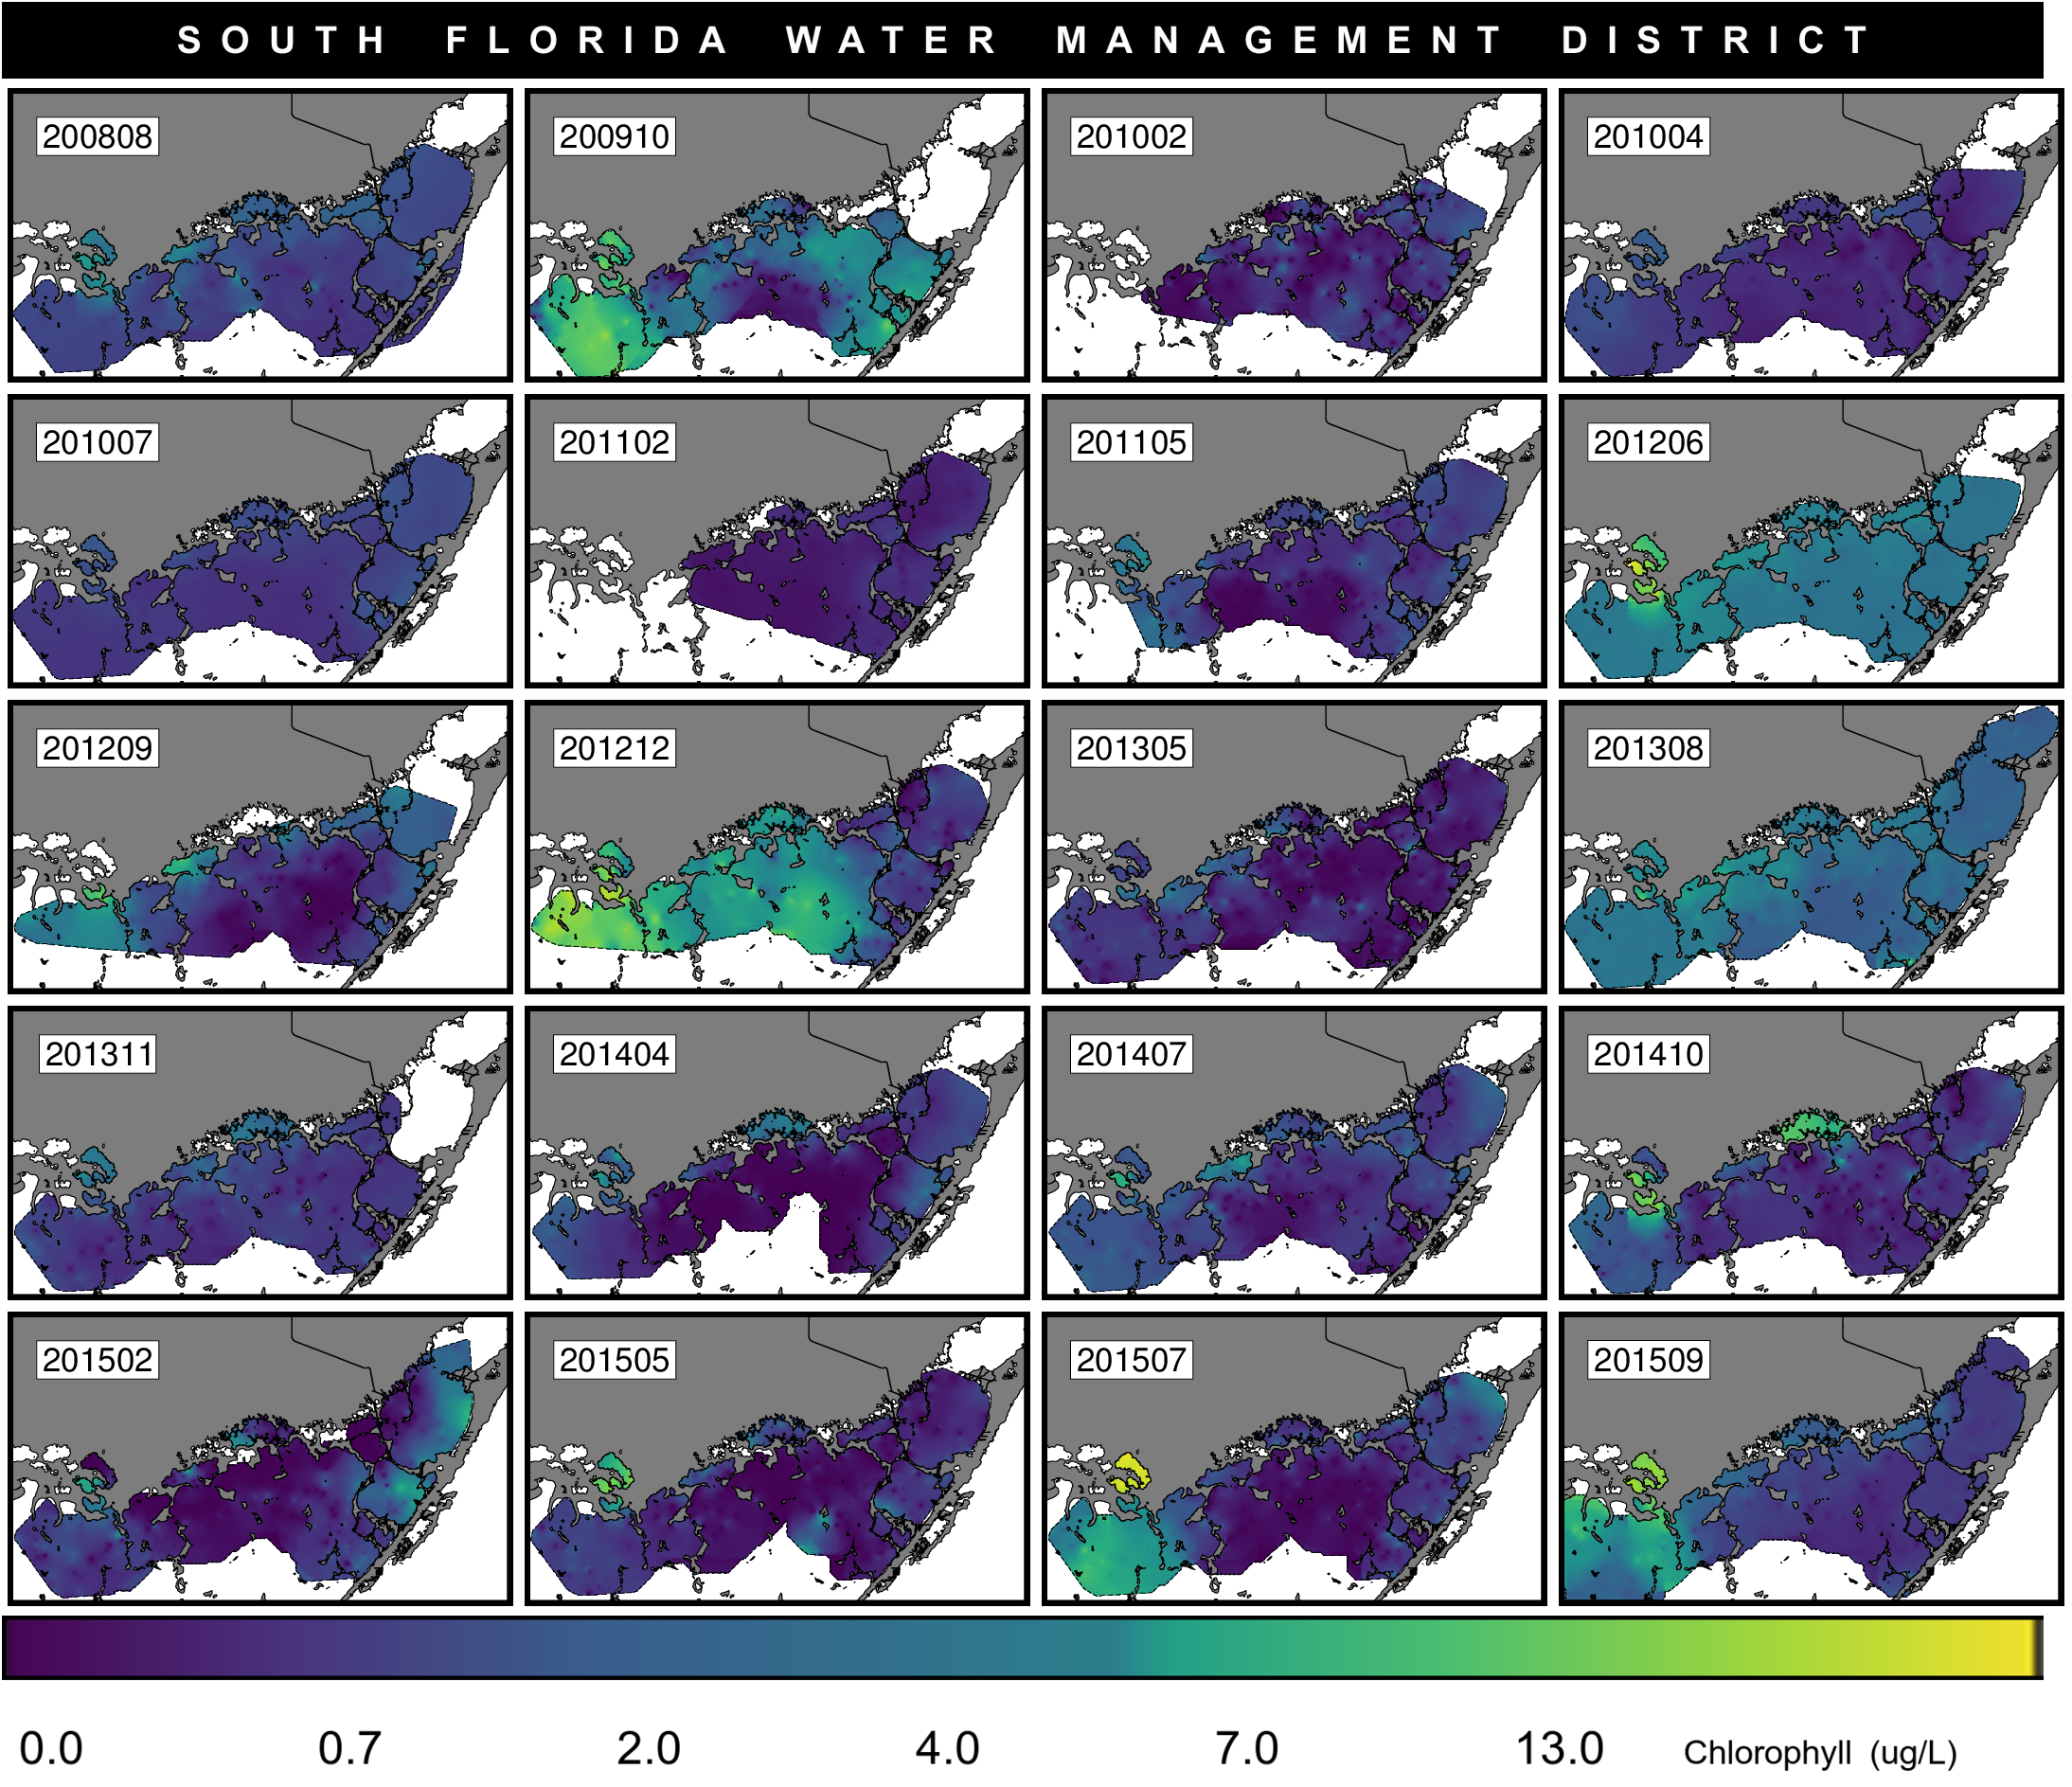
\includegraphics[height=7.6cm,keepaspectratio=true]{figures/multipanel.png}\\
		\end{centering}
		\end{frame}
		
		\begin{frame}{Spatio-Temporal Variability}
					\begin{center}
					\begin{tikzpicture}
						\node[anchor=south west,inner sep=0] at (0.7,0) {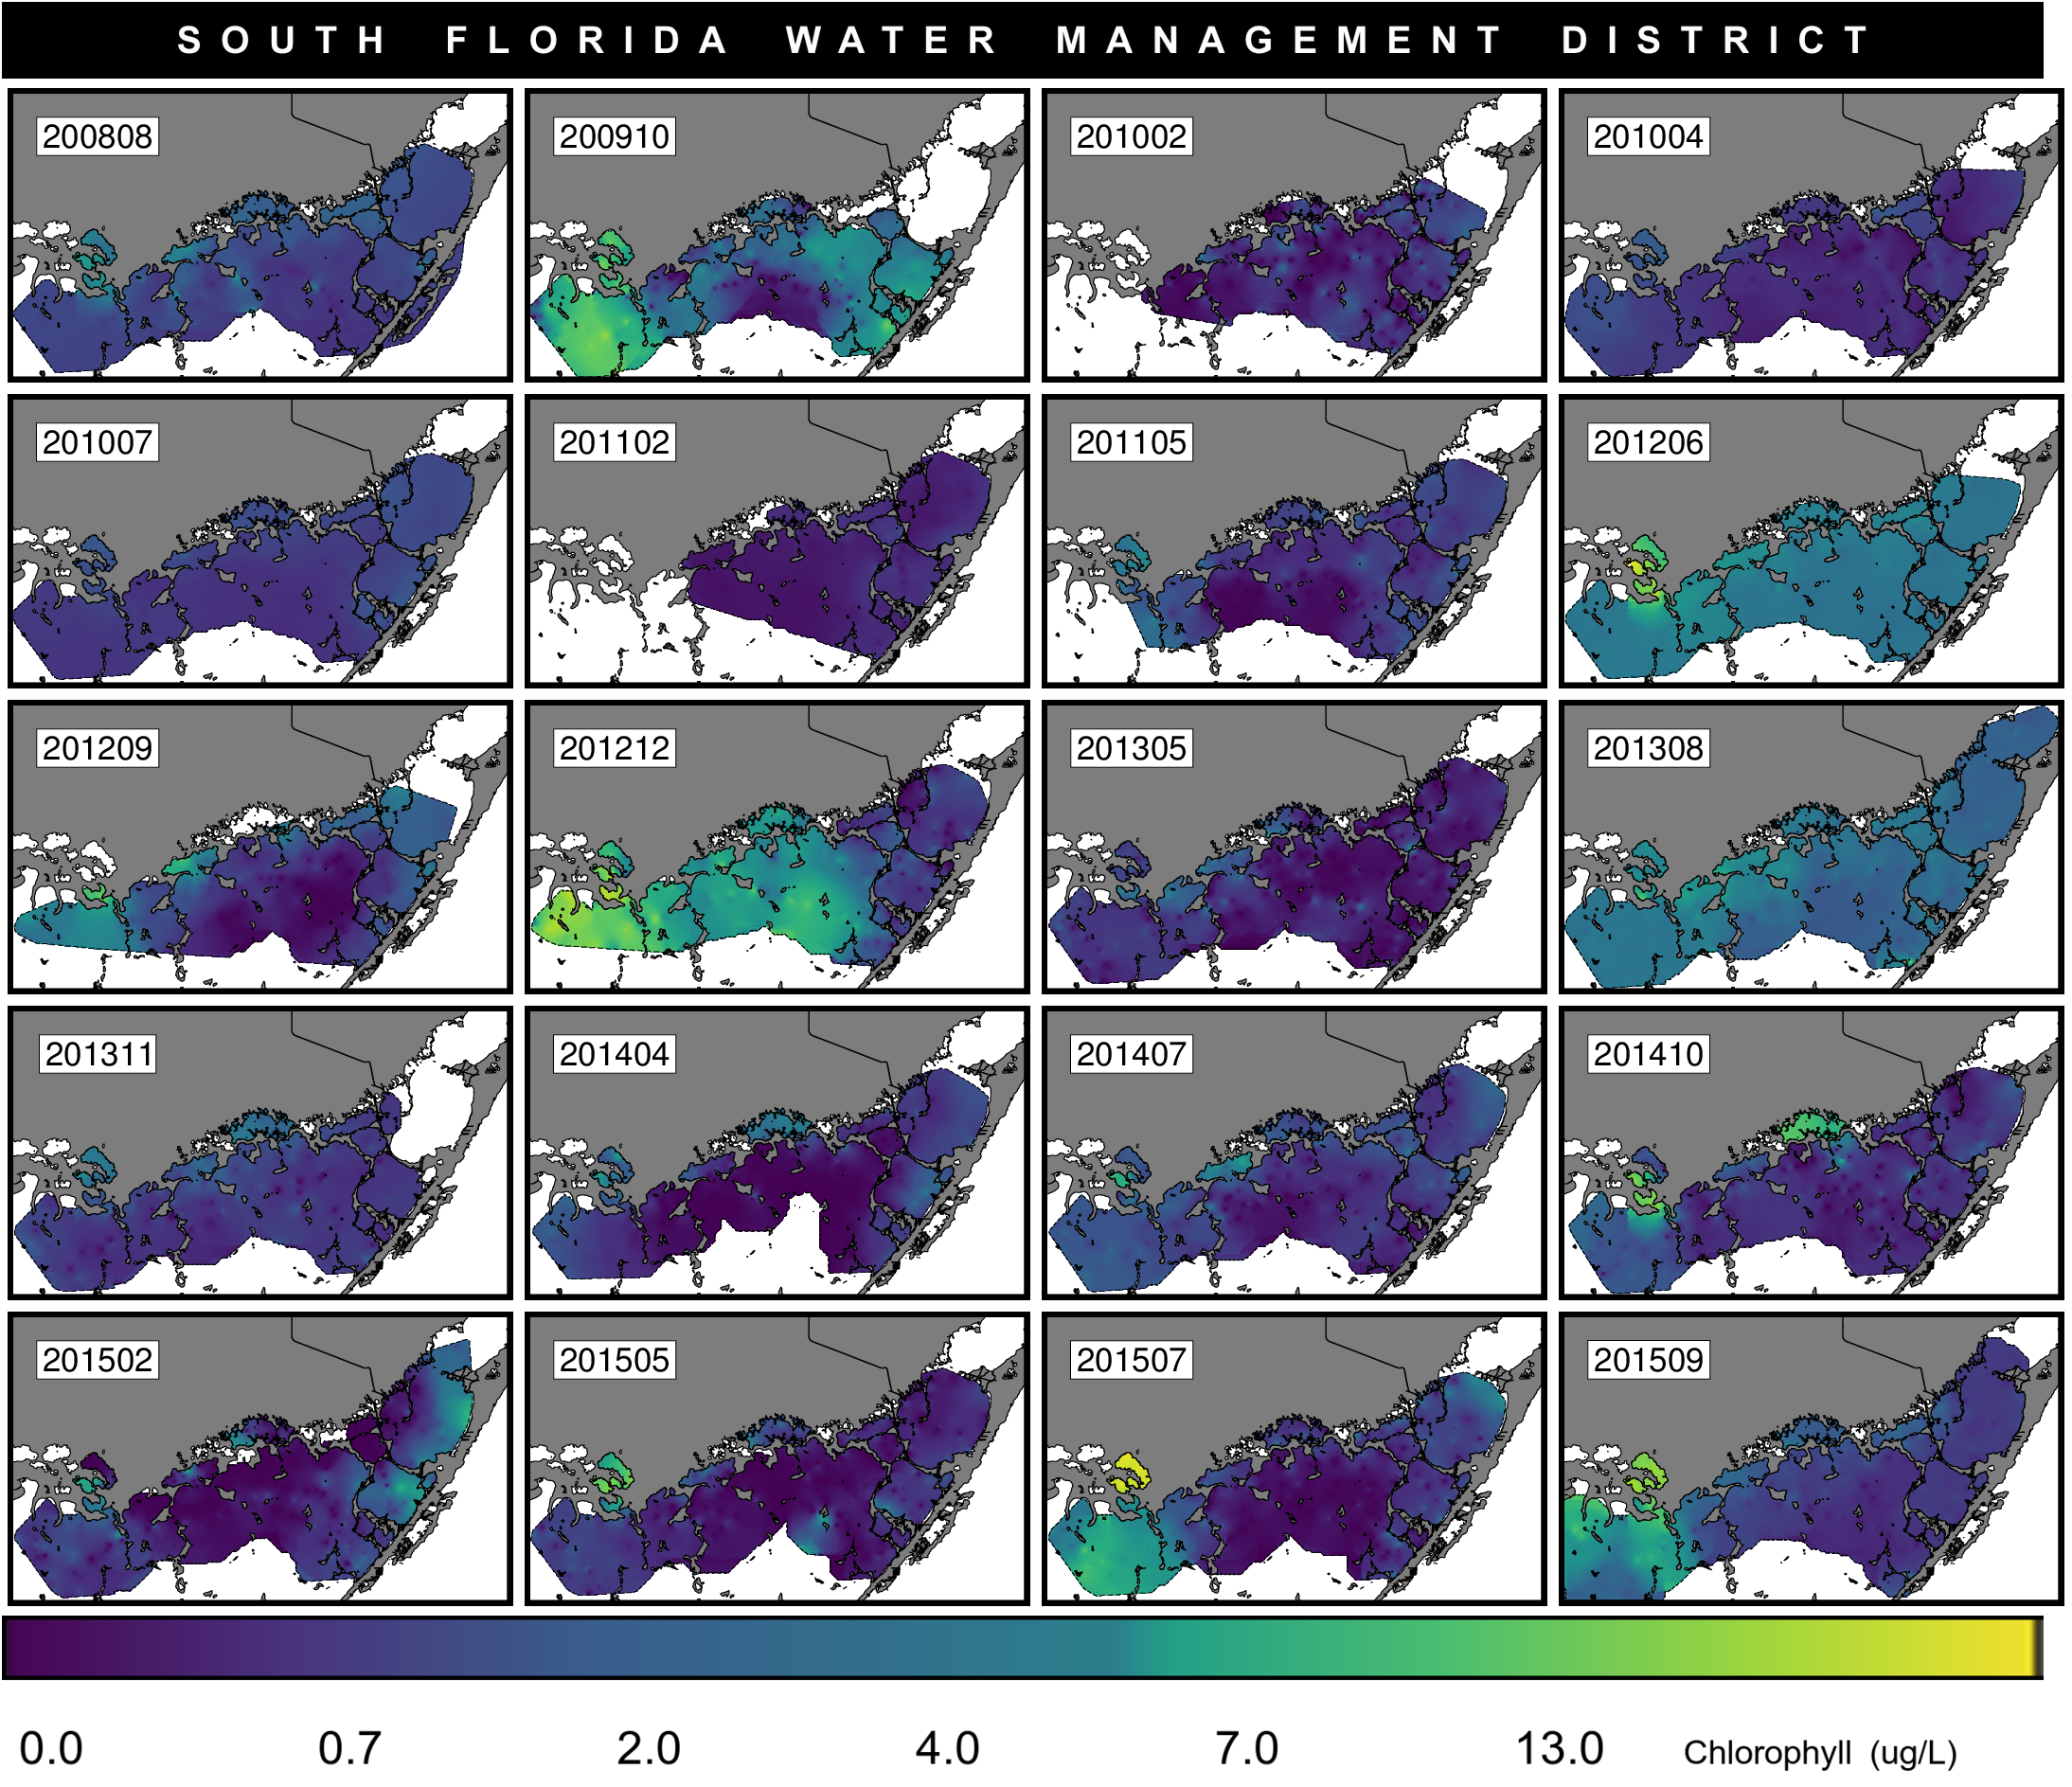
\includegraphics[height=7.6cm]{figures/multipanel.png}};
					% \draw[help lines,xstep=1,ystep=1](0.7,0) grid (10,7.6);
					% \foreach \x in {0.7,1.7,...,6.7}{ \node [anchor=north] at (\x,0) {\x};}
					% \foreach \y in {0,1,...,7}{ \node [anchor=east] at (0.7,\y) {\y};}
					 	\draw[red,thick, rounded corners](2.9,3.4) rectangle (5.1,4.6);
					 	\draw[red,thick, rounded corners](2.9,6) rectangle (5.1,7.2);
					\end{tikzpicture}
					\end{center}
			% \vspace{-3em}
		\end{frame}
		
		\begin{frame}{Spatial Variability}
		\vspace{-2em}
		\begin{columns}
		\begin{column}{6cm}
			\begin{center}
			\fbox{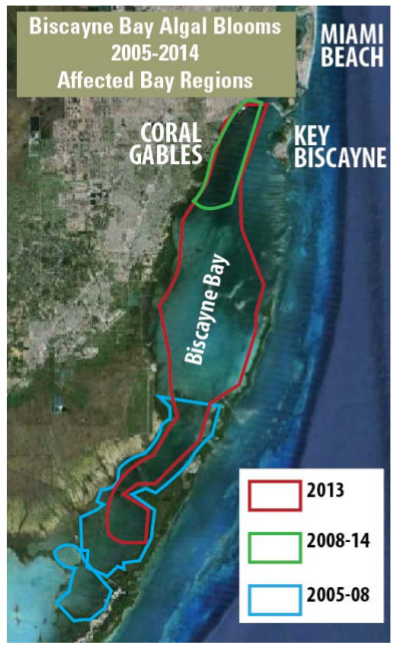
\includegraphics[height=7.5cm,keepaspectratio=true,clip=TRUE,trim=0mm 0mm 0mm -2mm]{images/flseagrant_biscayne-blooms.png}}\\
			\end{center}
		\end{column}
		\begin{column}{6cm}
			\begin{center}
			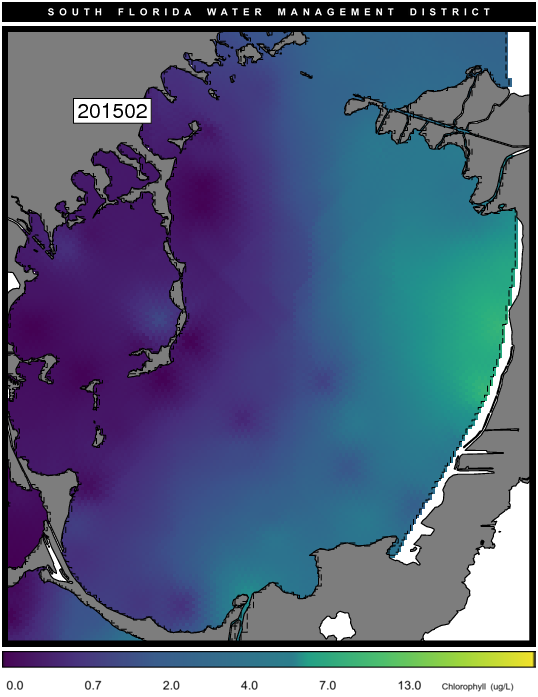
\includegraphics[height=7.8cm,keepaspectratio=true,trim= 0mm 0mm 0mm 9mm,clip=TRUE]{figures/barnes_chl.png}\\
			\end{center}
		\end{column}
		\end{columns}
		
		\end{frame}

\section{Resources}
\subsection{Resources}
\begin{frame}{Resources}
%The \tttext{ipdw} R package
  \centering
  \url{http://cran.r-project.org/package=ipdw}
%   \begin{verbatim}
%   "install.packages("ipdw")"
%   \end{verbatim}
  \begin{thebibliography}{10}
  \beamertemplatearticlebibitems
  \bibitem{stachetal2016}
	Stachelek~J.,C.~J.~Madden,S.~P.~Kelly,M.~Blaha (submitted). Fine-scale relationships between phytoplankton abundance and environmental drivers in Florida Bay, USA.
	\newblock \doublequoted{Estuaries and Coasts}
  \bibitem{stachmadden2015}
	Stachelek~J.,C.~J.~Madden. 2015. Application of Inverse Path Distance Weighting for high-density spatial mapping of coastal water quality patterns
	\newblock \doublequoted{Int. J. Geographical Information Science}
  \end{thebibliography}

	\begin{itemize}
		\item \url{stachel2@msu.edu}
	\end{itemize}
\end{frame}

\end{document}